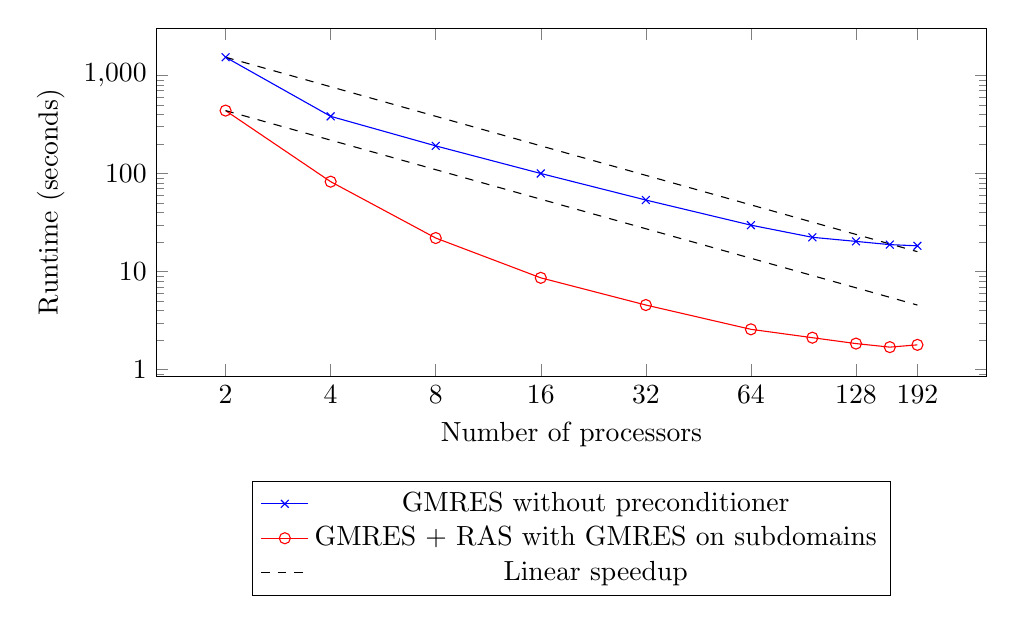
\begin{tikzpicture}
 \begin{axis}[
  height=6cm,
  width=\textwidth,
  xlabel=Number of processors,
  xtick={2, 4, 8, 16, 32, 64, 128, 192},
  xmode=log,
  ymode=log,
  log ticks with fixed point,
  ylabel=Runtime (seconds),
  legend style={
   at={(0.5, -0.3)},
   anchor=north
  }]
   \addplot[color=blue, mark=x] coordinates {
    (2, 1532.415986)
    (4, 382.7068273)
    (8, 191.2647738)
    (16, 100.056926)
    (32, 53.66010017)
    (64, 29.7611655)
    (96, 22.3732415)
    (128, 20.32742992)
    (160, 18.84248642)
    (192, 18.3280176)
   };
   \addlegendentry{GMRES without preconditioner}
   \addplot[color=red, mark=o] coordinates {
    (2, 437.742786)
    (4, 82.56500817)
    (8, 21.99554433)
    (16, 8.64097975)
    (32, 4.564814167)
    (64, 2.581634333)
    (96, 2.120893917)
    (128, 1.847387583)
    (160, 1.699225417)
    (192, 1.792736933)
   };
   \addlegendentry{GMRES + RAS with GMRES on subdomains}
   \addplot[color=black, domain=2:192, dashed] expression {
    1532.415986*2/x};
   \addlegendentry{Linear speedup}
   \addplot[color=black, domain=2:192, dashed] expression {
    437.742786*2/x};
 \end{axis}
\end{tikzpicture}
